\chapter{Introduction}

Acoustic signals are nowadays mostly used for military and research propose. Electromagnetic waves cant perpetuate water, so by the use of acoustic modems water can be used as a medium. Underwater vehicles need to be capable of communicate to either themselves or objects placed at the surface. Even though the throughput of these aucustic signals is way less than its electromagnetic counterpart, it still has the advantage to perpetuate fluids.\\


\section{Motivation}

Using water as a medium for localization signals can be somewhat sophisticated to implement and are therefore a challenging research topic. Due strong damping of the classic electromagnetic waves general technologies like GPS or GLONASS are not applicable in under water scenarios. \\
Acoustic transmission comes in handy in this case. Most systems use a vehicle which transmits acoustic beacons. These are then received by hydrophones placed at the surface. By estimating the travel times the distance between hydrophones and the underwater vehicle can be calculated. However, to let it localize itself, the reverse method is needed. Thus, anchors firmly fixed at the surface send their individual signals and the vehicle receives them.\\
Signals send by the anchors need to be separable but still observable. Therefore we need codes that are orthogonal towards each other but nonetheless posses clear auto-correlation. \\
This project dives into the mathematical details of pseudo.random maximum length sequence generation and signal processing. By the use of cross-correlation and auto-correlation the separation of signals can be implemented and evaluated. 

\section{Setup}

The setup consists of 4 Anchors fixed at the surface broadcasting different signals produced from an python program. Acoustic Modems use broadcast the transfer band signal into the water. At the beginning these 4 anchors need to be synchronized. A blueROV2 receives these signals under water and saves them. Afterward the saved signals are used in python to calculate the position of the ROV.
\begin{figure}[h]
	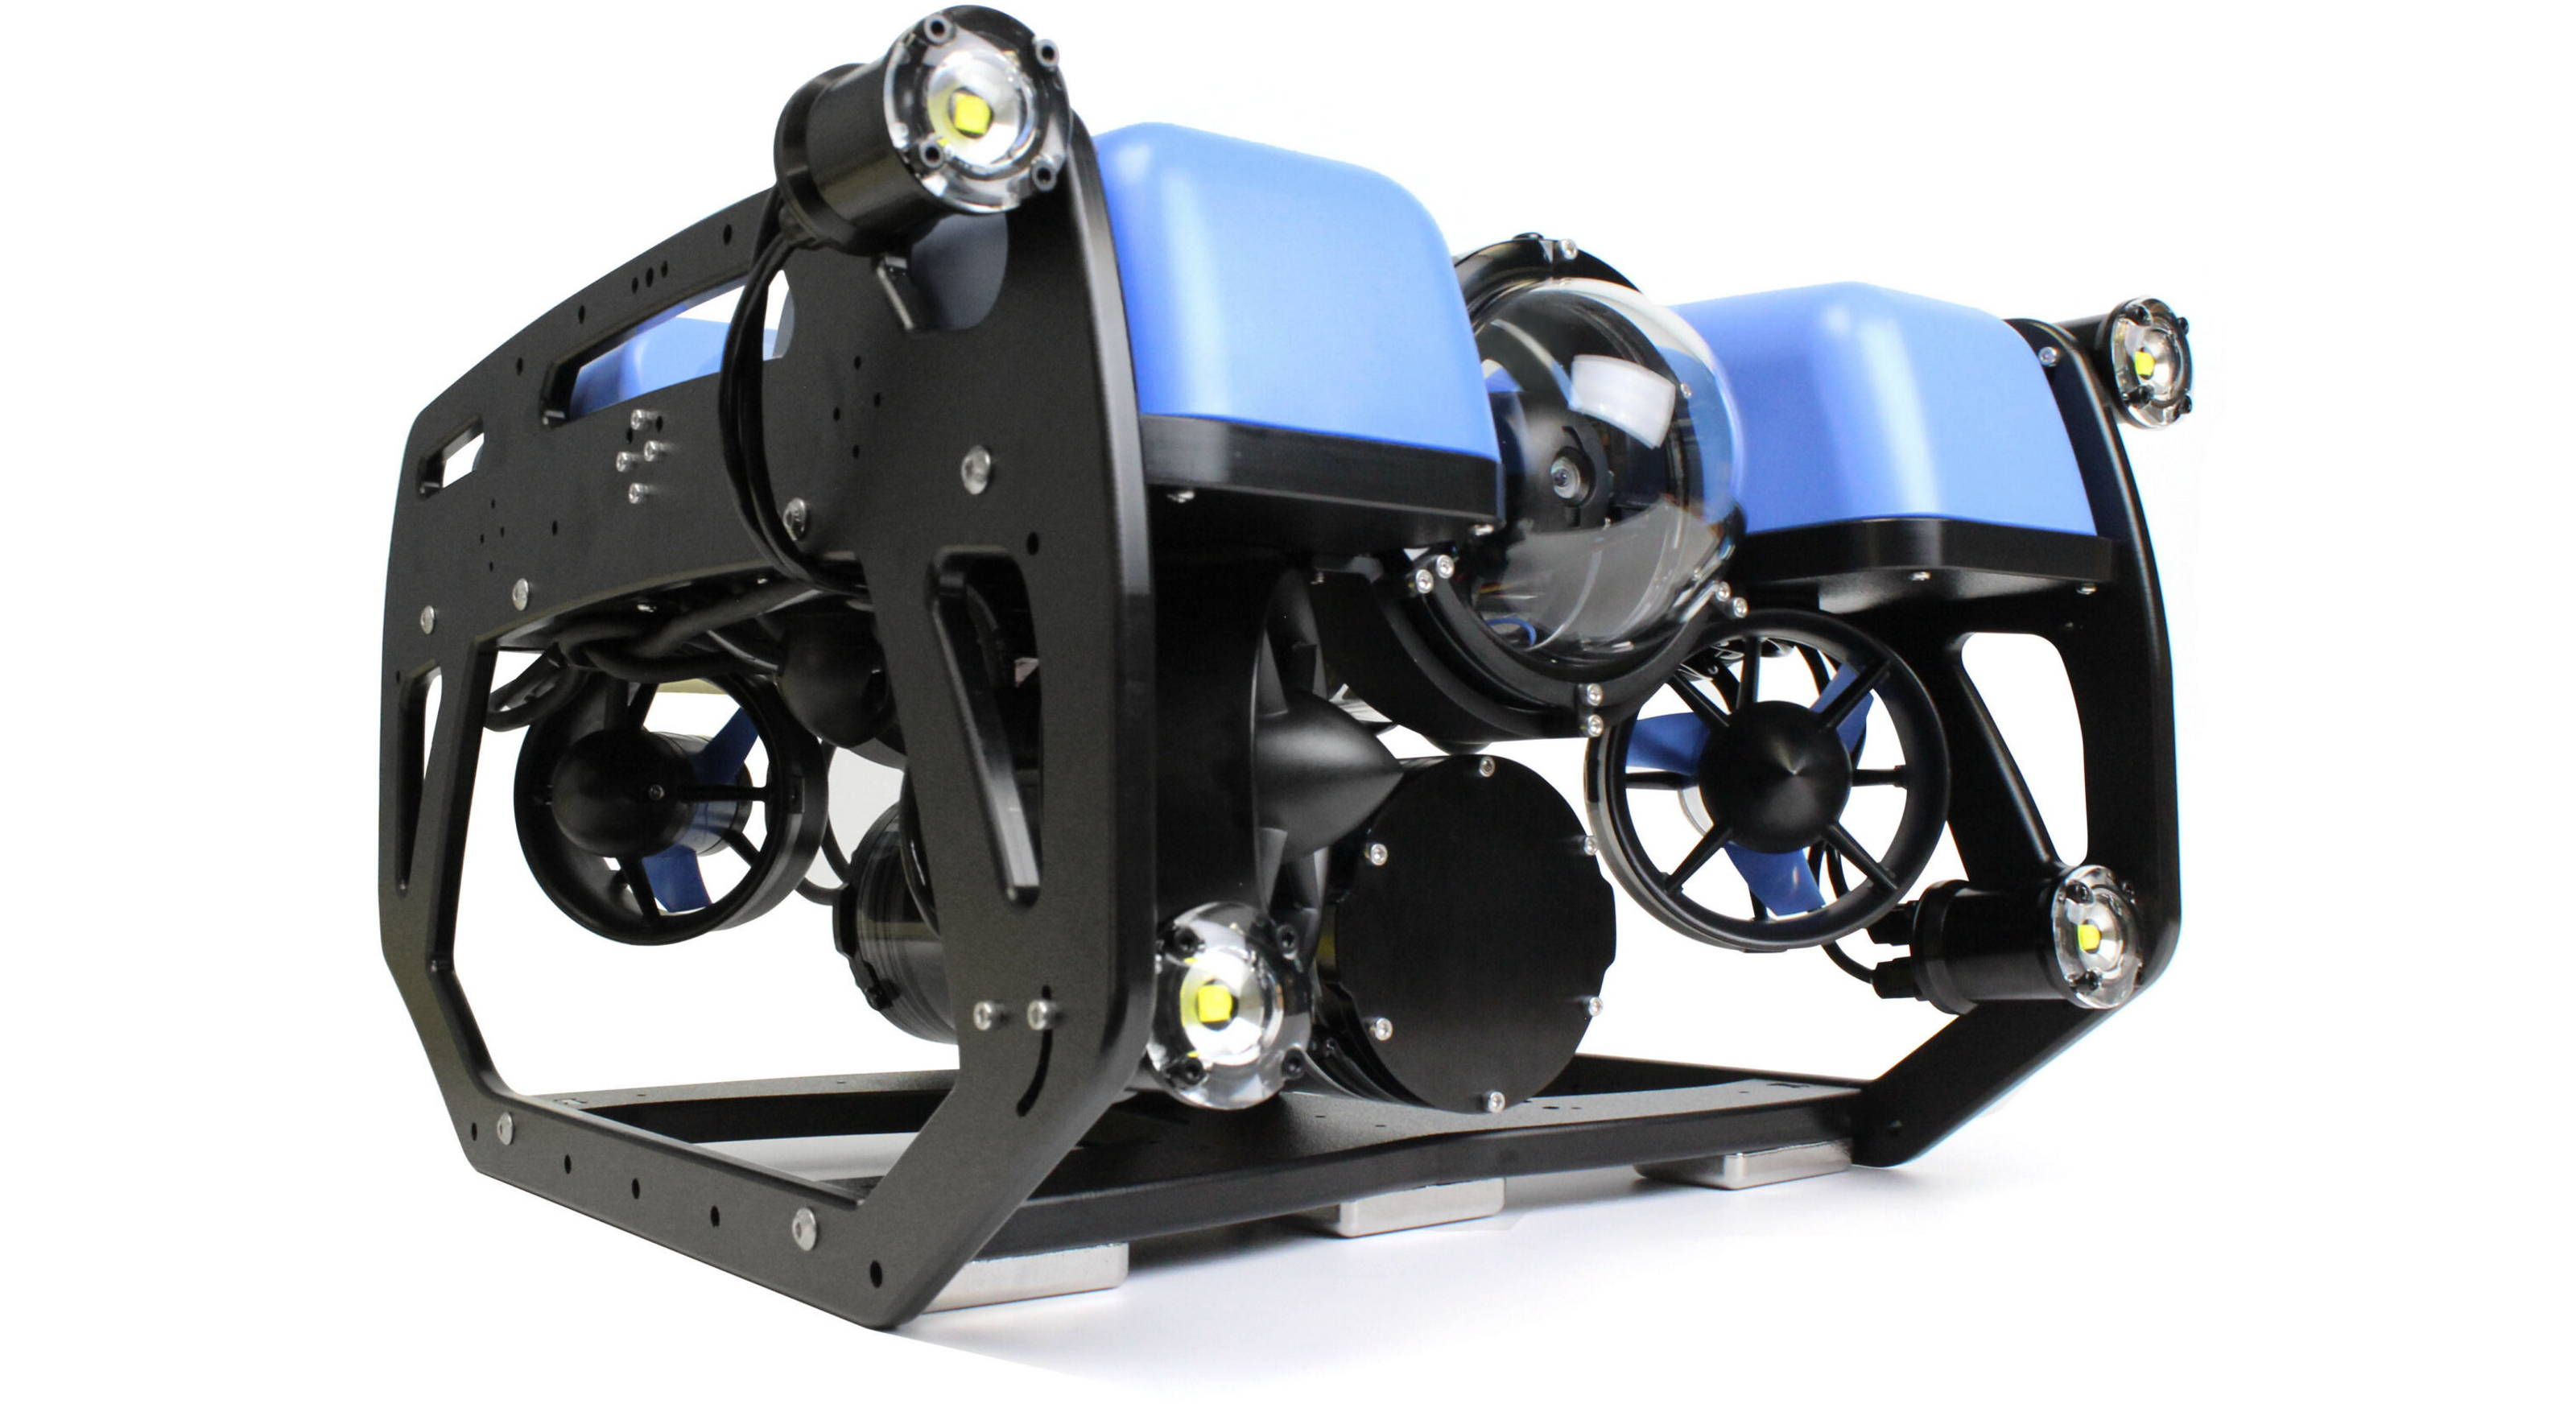
\includegraphics[height=5cm]{images/bluerov}
	
	\caption{BlueROV2 from Blue Robotics Inc}
	\label{fig:bode}
\end{figure}

\section{Principle}

To get the appropriate signals we need to apply certain signal processing steps. First the pseudo-random codes gets up-sampled and put though an cosine FIR filter to remove high frequencies from the base-band. The resulting signal is than shifted to the transfer band. Hereon either a custom delay is artificially added by zero padding for the simulation or is send by the acoustic modem. \\
Because of the advantageous properties of the used codes the different codes can be separated by cross-correlation by the not delayed versions. The cleaner the auto-correlation the higher are the peaks which are used to measure the initial delay. Method of peak detection may needed to filter out peaks caused from reflections.\\
